\documentclass{beamer}

% There are many different themes available for Beamer. A comprehensive
% list with examples is given here:
% http://deic.uab.es/~iblanes/beamer_gallery/index_by_theme.html
% You can uncomment the themes below if you would like to use a different
% one:
%\usetheme{AnnArbor}
%\usetheme{Antibes}
%\usetheme{Bergen}
%\usetheme{Berkeley}
%\usetheme{Berlin}
%\usetheme{Boadilla}
%\usetheme{boxes}
%\usetheme{CambridgeUS}
%\usetheme{Copenhagen}
%\usetheme{Darmstadt}
%\usetheme{default}
%\usetheme{Frankfurt}
%\usetheme{Goettingen}
%\usetheme{Hannover}
%\usetheme{Ilmenau}
%\usetheme{JuanLesPins}
%\usetheme{Luebeck}
\usetheme{Madrid}
%\usetheme{Malmoe}
%\usetheme{Marburg}
%\usetheme{Montpellier}
%\usetheme{PaloAlto}
%\usetheme{Pittsburgh}
%\usetheme{Rochester}
%\usetheme{Singapore}
%\usetheme{Szeged}
%\usetheme{Warsaw}

% Chinese display
\usepackage{CJKutf8}

% English? (cause Overleaf)
\usepackage[english]{babel}

% Flow Charts 
\usepackage{tikz}
\usetikzlibrary{shapes.geometric, arrows}
\tikzset{
	flowchartnode/.style = {minimum width=3cm, minimum height=1cm, text centered, draw=black},
	process/.style = {rectangle, flowchartnode, fill=orange!30},
	decision/.style = {diamond, flowchartnode, fill=green!30},
	io/.style = {trapezium, trapezium left angle=70, trapezium right angle=110, flowchartnode, fill=blue!30},
	line/.style = {draw, -latex'}
}

% Indexed letters inside circles
\newcommand\encircle[1]{%
  \tikz[baseline=(char.base)]{
  	\node[shape=circle,draw,inner sep=2pt] (char) {#1};}}

% Roman Numbers
\newcommand{\RNum}[1]{\uppercase\expandafter{\romannumeral #1\relax}}

% Tab
\newcommand{\tab}[1]{\hspace{.1\textwidth}\rlap{#1}}

% Divider
\newcommand{\divider}[1]{\noindent\rule{.9\textwidth}{1pt}}

% Set footnotetext without footnote mark
\let\thefootnote\relax\footnotetext{}

% Set caption with tiny size
\setbeamerfont{caption}{size=\tiny}

% Figure directory
\graphicspath{{fig/}}

% First page
\title[Progress Report]{Instant Auditing of Cloud Storage Access by Voting of Different Cloud Storages}
\author[Wei-Chih Chien]{Advicer : Gwan-Hwan Hwang \texorpdfstring{\\ Student : Wei-Chih Chien}{}}
\institute[NTNU CSIE CCLAB]{NTNU CSIE CCLAB}
\date{2016.05.24}

% Let every section start with outline
\AtBeginSection[]
{
  \begin{frame}<beamer>{Outline}
  	\tableofcontents[currentsection]
  \end{frame}
}

% Start content
\begin{document}
% Chinese display
\begin{CJK}{UTF8}{bkai}

\begin{frame}
  \titlepage
\end{frame}

\begin{frame}{Outline}
  \tableofcontents
\end{frame}

\section{Scenario}
\begin{frame}{Scenario}{Law Office}
	\alert{Advantage of Cloud Storage:}\\
	\textcolor{blue}{
		\hspace{.1\textwidth}Save money on hardware cost\\
		\hspace{.1\textwidth}Easily access files\\
		\hspace{.1\textwidth}...
	}
	\begin{center}
		
\includegraphics[width=.5\textwidth]{Scenario1}
	\end{center}
\end{frame}

\begin{frame}{Scenario (CON'T)}{Version Control}
	\begin{center}
		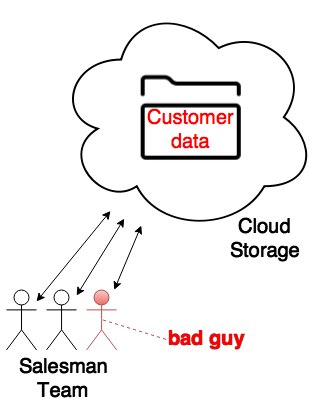
\includegraphics[width=.4\textwidth]{Scenario2}\\
		\textcolor{blue}{Always Get the Latest Version of Files.}
	\end{center}
\end{frame}

\begin{frame}{Scenario (CON'T)}{What if...}
	\begin{center}
		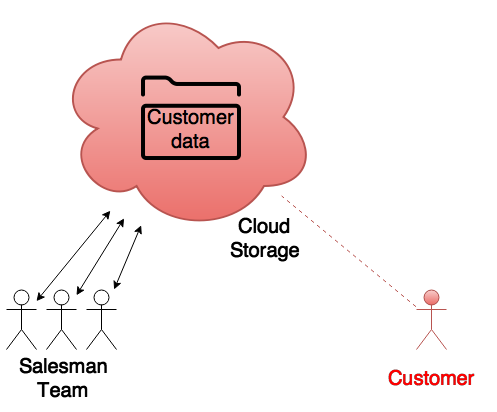
\includegraphics[width=.7\textwidth]{Scenario3}\\
		\textcolor{blue}{To request compensation, \alert{Cryptographic Proof} is necessary}
	\end{center}
\end{frame}

\section{Real-time Auditing Schemes}
\subsection{\small{Instant Auditing of Cloud Storage Access by Cache Partial Merkle tree}}
\begin{frame}{\normalsize{Instant Auditing of Cloud Storage Access by Cache Partial Merkle tree}}
{\tiny{2014 IEEE 6th International Conference on Cloud Computing Technology and Science}}
	\textcolor{blue}{Merkle Tree}\\
	~\\
	\begin{center}
		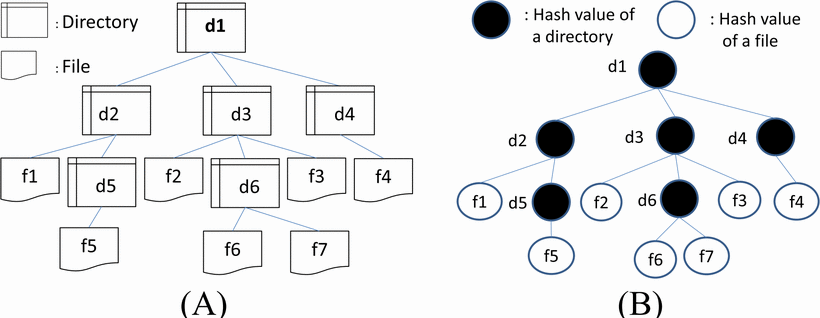
\includegraphics[width=.85\textwidth]{merkle_tree}
	\end{center}
\end{frame}

\begin{frame}{\normalsize{Instant Auditing of Cloud Storage Access by Cache Partial Merkle tree}}
{\tiny{2014 IEEE 6th International Conference on Cloud Computing Technology and Science}}
	\begin{center}
		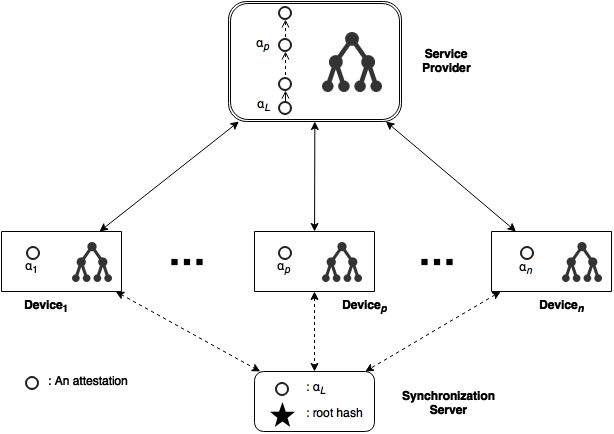
\includegraphics[width=.8\textwidth]{wei_shian}
	\end{center}
\end{frame}

\begin{frame}{Worst-case}
	\textcolor{blue}{若有個 device 很久沒有使用,在讀寫檔案前需要更新大量未做的動作\\
	~\\
	使用者將會明顯感受到漫長的等待時間}\\
	~\\
	~\\
	~\\
	\begin{center}
		\includegraphics[width=.5\textwidth]{worst_case}
	\end{center}
\end{frame}

\subsection{\small{My Method}}
\begin{frame}{My Method}
	\textcolor{blue}{Assumption: $\text{同時有 k 個 server 上同一 file 出問題的機率} \approx 0$}
	\begin{center}
		\alert{Service Providers are Independent Cloud}
		
\includegraphics[width=.7\textwidth]{wei_chih}
	\end{center}
\end{frame}

\begin{frame}{Comparison}
	\begin{itemize}
		\item \textcolor{blue}{Pros}
			\begin{enumerate}
				\item Device 不用儲存、也不用修改 Merkle tree, 既省空間又省時間
				\item 資料有多份備份
				\item 解決之前的 Worst-case
			\end{enumerate}
		~\\
		\item \textcolor{red}{Cons}
			\begin{enumerate}
				\item 需要傳送多份 Request, 處理多份 Response
			\end{enumerate}
	\end{itemize}
\end{frame}

\section{Protocol Detail}
\subsection{Flowchart}
\begin{frame}{Flowchart}
	\begin{center}
		\resizebox{!}{.6\textwidth}
		{%
			\begin{tikzpicture}[node distance=2cm]
				% Define flow charts' component
				\node (init) [process] {Initial};
				\node (lock) [process, below of=init] {Lock};
				\node (twostep) [process, below of=lock] {2-step Handshake};
				\node (twostep_left) [process, left of=twostep, xshift=-2cm] {2-step Handshake};
				\node (twostep_right) [process, right of=twostep, xshift=2cm] {2-step Handshake};
				\node (voting) [decision, below of=twostep] {Voting};
				\node (store) [process, below of=voting, yshift=-0.5cm] {Store ACK};
				\node (update) [io, below of=store, align=center] {File \\ Transmit};
				\node (auditing) [process, right of=update, xshift=2.5cm] {Auditing};
				\node (unlock) [process, left of=store, xshift=-4cm] {Unlock};

				% Define flow charts' link
				\path [line](init) -- (lock);
				\path [line](lock) -- (twostep);
				\path [line](lock) -- (twostep_left);
				\path [line](lock) -- (twostep_right);
				\path [line](twostep) -- (voting);
				\path [line](twostep_left) -- (voting);
				\path [line](twostep_right) -- (voting);
				\path [line](voting) -- node[anchor=east] {k個以上的}
									    node[anchor=west] {ACK相同} (store);
				\path [line](voting) -| node[anchor=west] {ACK不相同} (auditing);
				\path [line](store) -- (update);
				\path [line](store) -- (unlock);
				\path [line](unlock) |- (lock);
			\end{tikzpicture}%
		}
	\end{center}
\end{frame}

\subsection{Download \& Upload}
\begin{frame}{Download \& Upload}
	\centering
	\textcolor{blue}{\textbf{Request \& Response}}\\
	~\\
	~\\
	\begin{minipage}{.45\textwidth}
        \includegraphics[width=1\textwidth]{2_step_handshake}
    \end{minipage}%
	\begin{minipage}{.55\textwidth}
    	\footnotesize
		\centering
		\begin{equation} \label{eq1}
                \begin{split}
                        \textcolor{blue}{REQ} & = (OP, [OP]_{pri(D)}) \\
                        OP & = (TYPE, PATH, HASH) \\
                \end{split}
        \end{equation}
        \divider{}\\
        \begin{equation} \label{eq2}
                \begin{split}
                        \textcolor{red}{ACK} & = (RESULT, REQ,\\
                        & \tab{}\tab{}[RESULT, REQ]_{pri(S)}) \\
                        RESULT & = (roothash, filehash)
                \end{split}
        \end{equation}
        \textcolor{red}{\textbf{collect ACKs and voting}}
    \end{minipage}%
\end{frame}

\begin{frame}{if Operation is UPLOAD}
	\centering
	\textcolor{blue}{\textbf{Server Update Merkle tree}}\\
	~\\
	~\\
	\begin{center}
		\includegraphics[width=.65\textwidth]{update_merkle_tree}
	\end{center}
\end{frame}

\begin{frame}{File Transmit}
	\begin{center}
		\includegraphics[width=.65\textwidth]{file_transmit}
	\end{center}
\end{frame}

\subsection{Audit}
\begin{frame}{Audit}
	\textcolor{blue}{$\because$ ACK 中有 roothash\\
	$\therefore$ 新的 request 之前,所有的檔案都經過檢查,沒有問題}\\
	~\\	
	\begin{block}{}
		\centering
		device request $OP_i$,收到回傳的 $ACK_i$\\
		發現 $Server_p$ 的 ACK 有錯誤,因此向 $Server_p$ 稽核\\
		~\\
		device 向 $Server_p$ 索取 $MT_{i-1}$\\
		($MT_{i-1}$ 為執行 $OP_i$ 之前的 Merkle tree)
	\end{block}
	\begin{alertblock}{\encircle{1}\encircle{2} 兩點有一個出錯就能確定 $Server_p$ 出錯}
		\encircle{1} device 檢查 $MT_{i-1}$ 的 roothash 應和 $ACK_{i-1}$ 中的 roothash 一樣\\
		\encircle{2} device 以 $OP_i$ 中的 hash value 來更新 $MT_{i-1}$,\\
		\tab{}更新後的 roothash 應和 $Server_p$ 現在的 roothash 相同
	\end{alertblock}	
\end{frame}

\section{Experimental Results}
\begin{frame}{Experimental Results}
	\begin{table}[]
		\scriptsize
		\centering
		\begin{tabular}{crccr}
			  & Size    & File  & Directory & Merkle tree Size \\
			  &			&		&		    &                  \\
			A & 777 MB  & 48    & 6         & 5.4 KB           \\
			B & 145 MB  & 54198 & 188       & 5.08 MB          \\
			C & 5.95 GB & 45089 & 1459      & 4.37 MB          \\
		\end{tabular}
        
		\caption{GENERATE MERKLE TREE'S TIME (IN SEC.)}
		\begin{tabular}{|c|r|c|c|c|}
			\hline
			   &             & A      & B       & C       \\ \hline
               &             &        &		    &		  \\ \hline
			   & Generate    & 14.876 & 61.176  & 198.405 \\ \cline{2-5} 
			PC & Serialize   & 0.040  & 0.756   & 0.670   \\ \cline{2-5} 
			   & Deserialize & 0.009  & 0.299   & 0.295   \\ \hline
		   	   &             &        &         &         \\ \hline
			   & Generate    & 6.821  & 144.267 & 620.151 \\ \cline{2-5} 
			VM & Serialize   & 0.011  & 0.343   & 0.299   \\ \cline{2-5} 
			   & Deserialize & 0.015  & 1.016   & 0.860   \\
			\hline
		\end{tabular}
	\end{table}
\end{frame}

\begin{frame}{Experimental Results}
	\scriptsize
	\begin{table}
    	\large
		\centering
		\caption{THE EXECUTION TIME OF \alert{UPLOAD} OPERATIONS (IN SEC.) (Account C)}
		\begin{tabular}{lccc}      	
            Test File Size & Non POV  & Voting   & 2014 CloudCom \\ \hline
            $<$ 10 KB      & 0.005518 & 0.037380 & 0.218630      \\ \hline
            $<$ 100 KB     & 0.015352 & 0.039608 & 0.232741      \\ \hline
            $<$ 1 MB       & 0.056828 & 0.105343 & 0.272903      \\ \hline
            $<$ 10 MB      & 0.359668 & 0.391630 & 0.567197      \\
		\end{tabular}
	\end{table}
    \begin{alertblock}{2014 CloudCom Worst-case}
    	\normalsize
    	\tab{} Synchronize (HashChain length = 100) cost \textcolor{red}{0.595 sec}. \\
        \tab{} Synchronize (HashChain length = 1000) cost \textcolor{red}{5.54 sec}.
    \end{alertblock}
\end{frame}

\begin{frame}{Experimental Results}
	\scriptsize	
	\begin{table}[]
    	\large
		\centering      
		\caption{THE EXECUTION TIME OF \alert{DOWNLOAD} OPERATIONS (IN SEC.) (Account C)}
		\begin{tabular}{lccc}      	
            Test File Size & Non POV  & Voting   & 2014 CloudCom \\ \hline
            $<$ 10 KB      & 0.213026 & 0.036708 & 0.231693      \\ \hline
            $<$ 100 KB     & 0.219071 & 0.074291 & 0.237524      \\ \hline
            $<$ 1 MB       & 0.258437 & 0.191194 & 0.271910      \\ \hline
            $<$ 10 MB      & 0.548203 & 1.033431 & 0.551122      \\
		\end{tabular}
	\end{table}
    \tab{} \textcolor{red}{(數據有問題需更正)}
    \begin{alertblock}{2014 CloudCom Worst-case}
    	\normalsize
    	\tab{} Synchronize (HashChain length = 100) cost \textcolor{red}{0.827 sec}. \\
        \tab{} Synchronize (HashChain length = 1000) cost \textcolor{red}{7.871 sec}.
    \end{alertblock}
\end{frame}

\begin{frame}
	\begin{center}
		
\includegraphics[width=\textwidth]{thank_you.jpg}
	\end{center}	
\end{frame}

\end{CJK}
\end{document}
